On the same axes as in the previous part, plot the vectors $\boldsymbol{SSSSn}$ and $\boldsymbol{SSSSz}$ using MATLAB.

\begin{solution} \
    \begin{lstlisting}[language=Matlab]
n = [-1; 1];
z = [-1; 1.01];
S = [2 1; 1 2];

Sn = S*n;
Sz = S*z;
SSn = S*S*n;
SSz = S*S*z;
SSSn = S*S*S*n;
SSSz = S*S*S*z;
SSSSn = S*S*S*S*n;
SSSSz = S*S*S*S*z;

hold on
quiver(0, 0, n(1), n(2));
quiver(0, 0, z(1), z(2));
quiver(0, 0, Sn(1), Sn(2));
quiver(0, 0, Sz(1), Sz(2));
quiver(0, 0, SSn(1), SSn(2));
quiver(0, 0, SSz(1), SSz(2));
quiver(0, 0, SSSn(1), SSSn(2));
quiver(0, 0, SSSz(1), SSSz(2));
quiver(0, 0, SSSSn(1), SSSSn(2));
quiver(0, 0, SSSSz(1), SSSSz(2));

legend('n', 'z', 'Sn', 'Sz', 'SSn', 'SSz', 'SSSn', 'SSSz')
hold off
    \end{lstlisting}
    \begin{center}
        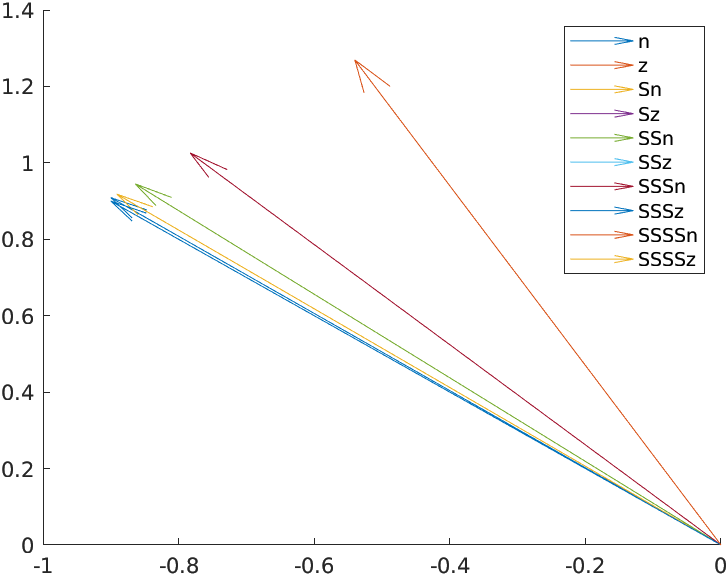
\includegraphics[width=0.7\textwidth]{img/e8p5.png}
    \end{center}
\end{solution}